% Universidade Federal do Rio Grande do Norte
% Programa de Pos-Graduacao em Engenharia Eletrica e de Computacao
% Lista 1 - Questao 1
% Autores: Anna Giselle Camara Dantas Ribeiro
%          Cristiano Gurgel de Castro
%          Diogo Leite Reboucas
%          Thiago Medeiros Barros

% Revisado em 14/06/2010 16:29 por crisgc

\chapter*{Questão 2}

\textit{Um sistema com realimentação unitária tem a seguinte função de
transferência de malha aberta:}

\begin{flalign*}
G(s) = \frac{s+r}{(s+p)(s+q)}
\end{flalign*}

\noindent \textit{em que $3 \leq p \leq 5$, $0 \leq q \leq 1$ e $1 \leq r \leq
2$.  Selecione os parâmetros (todos reais) de um controlador atraso-avanço de
fase, de forma que o sistema em malha fechada tenha um desempenho robusto. Faça
simulações no \Matlab\ para comprovar o desempenho do sistema.}

\vspace{0.5cm}

\noindent{\bf Resolução:}

\vspace{0.25cm}

Para efeitos de análise e projeto dos controladores, foram utilizados os valores
médios de cada um dos parâmetros, a saber $\vmedio{r} = 1.5$, $\vmedio{p} = 4$ e
$\vmedio{q} = 0.5$, sendo a função de transferência de malha aberta escrita
conforme Eq. \ref{eq:q2:gma}.

\begin{flalign}
\vmedio{G}(s) & = \frac{s+\vmedio{r}}{(s+\vmedio{p})(s+\vmedio{q})}  =
\frac{s+1.5}{(s+4)(s+0.5)} = {\frac{1.5+s}{2+4.5s+s^{2}}} \label{eq:q2:gma}
\end{flalign}

O lugar geométrico das raízes para esse sistema é mostrado na Fig.
\ref{fig:q2:rlocus_gma}.

\begin{figure}[htb]
\centering
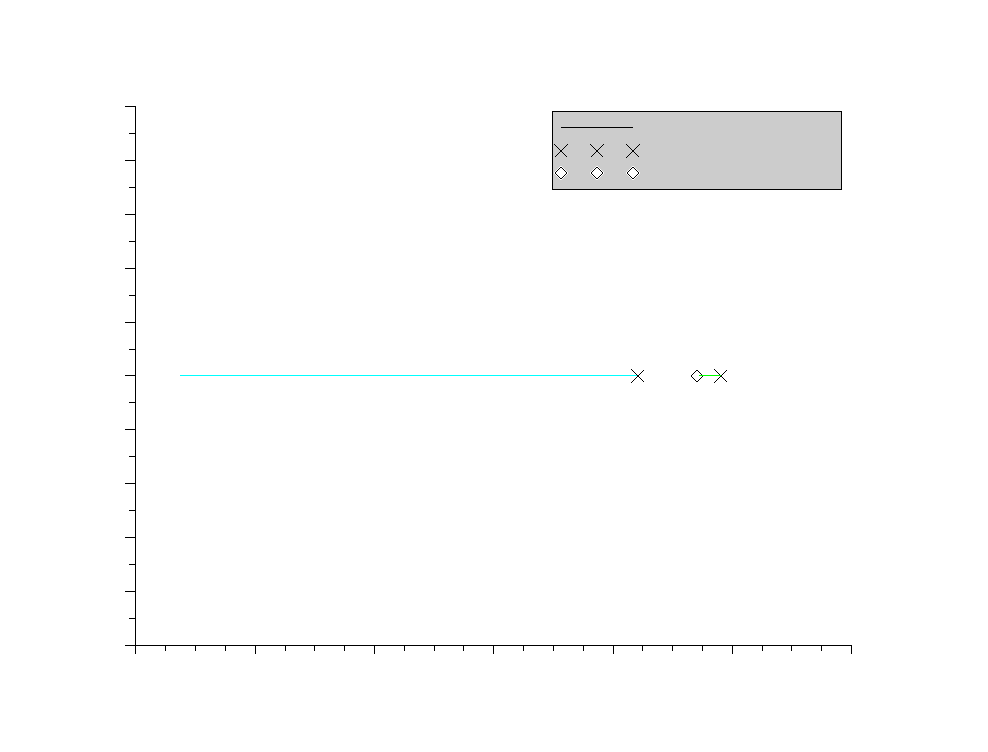
\includegraphics[width=0.95\textwidth]{imgs/questao2/rlocus_gma}
\caption{Lugar das raízes para os valores médios ($\vmedio{G}(s)$).}
\label{fig:q2:rlocus_gma}
\end{figure}

% TODO(crisgc): colocar diagrama de bloco com a malha fechada
Inicialmente a malha foi fechada e sua robustez foi testada segundo os
polinômios de Kharitonov. A função de transferência em malha fechada é mostrada
abaixo:

\begin{flalign}
G_{\text{MF}}(s) & = \frac{s+r}{(s+p)(s+q) + s+r} =
\frac{s+r}{s^{2}+\underbrace{(p+q+1)}_{a_1}s +
\underbrace{pq+r}_{a_0}} \nonumber \\
\vmedio{G_{\text{MF}}}(s) & = {\frac{1.5+s}{3,5+5.5s+s^{2}}} =
\frac{1.5+s}{(s+4.7656)(s+0.7344)} \quad
\bigtriangleup
\quad \text{Para os valores médios} \label{eq:q2:gmf}
\end{flalign}

Analisando a função de transferência de malha fechada, tem-se que:

\begin{flalign*}
a_0 &= pq+r & \alpha_0 & = \mymin{p}\mymin{q} + \mymin{r} = 1 \quad 
&\beta_0 &= \mymax{p}\mymax{q} + \mymax{r} = 7 \\
a_1 &= p + q + 1 & \alpha_1 &= \mymin{p} + \mymin{q} + 1 = 4 \quad
&\beta_1 &=\mymax{p} + \mymax{q} + 1 = 7
\end{flalign*}

Os quatro polinômios retirados do \textit{Teorema de Kharitonov} para o teste da
estabilidade são, então:

\begin{flalign*}
q_0 & = \alpha_0 + \alpha_1s + s^{2} = 1 + 4s + s^{2} = 
                                       (s + 3,7321)(s + 0,2679)\\
q_1 & = \alpha_0 + \beta_1s + s^{2} = 1 + 7s + s^{2} = 
                                      (s + 6,8541)(s + 0,1459)\\
q_2 & = \beta_0 + \alpha_1s + s^{2} = 7 + 4s + s^{2} = 
                                      (s + 2 + 1,7321i)(s + 2 -1,7321i)\\ 
q_3 & = \beta_0 + \beta_1s + s^{2} = 7 + 7s + s^{2} = (s + 5,7913)(s + 1,2087)\\
\end{flalign*}

Assim, como nenhum polo do sistema está situado no semiplano direito, ou seja,
todos os polos tem parte real negativa, o sistema é estável para qualquer valor
dos parâmetros dentro do seus intervalos de variação. Dessa maneira foi obtido o
valor final aproximado a partir do {\it teorema do valor final}:

\begin{flalign*}
\lim_{t \tende \infty}{y(t)} & = \lim_{s \tende 0}sY(s) \\
Y(s) & = R(s)\vmedio{G_{\text{MF}}}(s) = \frac{1}{s}\frac{1.5+s}{3.5+5.5s+s^{2}} \\
\lim_{t \tende \infty}{y(t)} & =  \lim_{s \tende
0}s\frac{1}{s}\frac{1.5+s}{3.5+5.5s+s^{2}} = \frac{1.5}{3.5} = \frac{3}{7}
\approx 0.429
\end{flalign*}

\noindent observa-se que esse valor obtido está condizente com a simulação, conforme Fig.
\ref{fig:q2:resposta_gmf}.

\begin{figure}[htb]
\centering
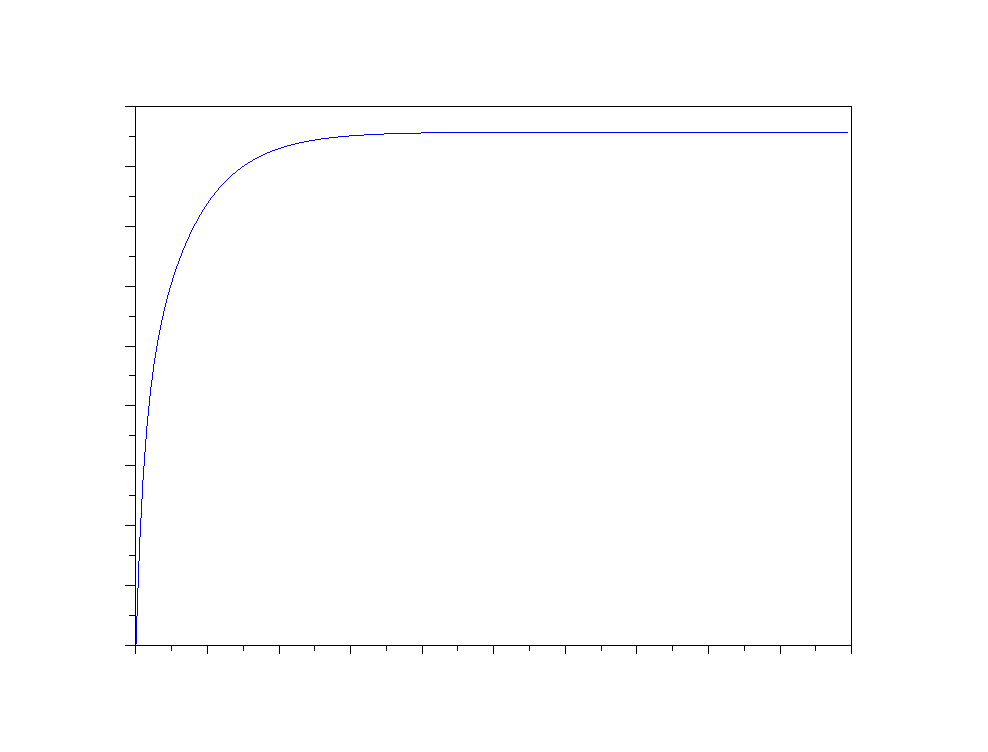
\includegraphics[width=0.95\textwidth]{imgs/questao2/resposta_gmf}
\caption{Resposta do sistema em malha fechada ao degrau unitário.}
\label{fig:q2:resposta_gmf}
\end{figure}

Sob o ponto de vista do projeto do controlador, o primeiro passo foi o de se
projetar um controlador em atraso de fase que, segundo \citeasnoun{dorf:2009} e
\citeasnoun{maitelli2002}, tem por objetivo melhorar o erro de regime a uma
entrada em degrau. A constante de erro de posição do sistema que foi obtida é
dada por $K_{p} = G(0) = 0.75$, o que resulta no erro de regime previamente
calculado. 

Adotando uma tolerância do erro de regime de aproximadamente $1\%$, foi
projetado um compensador de modo que $K'_p = 100$. Uma vez que o controlador em
atraso de fase possui função de transferência dada pela Eq. \ref{eq:comp_atras},

% TODO(crisgc): Colocar a figura da resposta em malha fechada simples
\begin{flalign}
G_c(s) & = k_c \frac{s+z_c}{s+p_c} \quad \text{onde} \quad |z_c| > |p_c|
\label{eq:comp_atras}
\end{flalign}

\noindent para obter a constante de erro desejada tem-se então que:

\begin{flalign}
\underbrace{K'_{p}}_{100} & = G_c(0)G(0) = G_c(0)K_{p} = k_c \frac{z_c}{p_c}
\underbrace{K_{p}}_{0.75} \nonumber \\
k_c \frac{z_c}{p_c}& = \frac{100}{0.75} = \frac{400}{3} \approx 133.333
\label{eq:q2:comp_atraso}
\end{flalign}

Como o polo dominante do sistema de malha aberta está localizado em $-0.5$ (Eq.
\ref{eq:q2:gma}) o zero do controlador foi alocado à sua direita, para que a
interferência no regime transitório não seja muito significante. Fez-se então
$z_c = 0.3$, e, optando em um primeiro momento por não adicionar o ganho no
controlador de tal maneira que $k_c = 1$, o polo, calculado a partir de
\ref{eq:q2:comp_atraso} foi então $p_c = 0.0022$. 

A função de transferência em malha fechada do sistema mostrado na Fig.
\ref{fig:q2:malha_comp} pode ser obtida através da redução do diagrama de
blocos.

\begin{figure}[htb]
\centering
\scalebox{0.7}{\input{imgs/questao2/compensador_malha.pstex_t}}
\caption{Diagrama de blocos para o sistema com o compensador.}
\label{fig:q2:malha_comp}
\end{figure}

Assim sendo:

\begin{flalign}
G_\text{cMF}(s) & = \frac{G_c(s)G(s)}{1 + G_c(s)G(s)} =
\frac{k_c(s+z_c)(s+r)}{k_c(s+z_c)(s+r) + (s+p)(s+q)(s+p_c)} \nonumber \\
& = \frac{k_cs^{2} + k_c(z_c + r)s + k_crz_c}{s^{3} + \underbrace{[k_c + p_c +
(p+q)]}_{a_2}s^{2} +
\underbrace{[k_c(r+z_c) + p_c(p+q)+pq]}_{a_1}s + \underbrace{rz_c + pqp_c}_{a_0}
} \label{eq:q2:testeKharitonov}
\end{flalign}

A estabilidade do sistema foi testada segundo o \textit{teorema de Kharitonov}.
Os quatro polinômios obtidos para os valores calculados do controlador, a saber
$z_c = 0.3$, $k_c = 1$ e $p_c = 0.0022$, foram:

\begin{flalign*}
q_1(s) & = 0.3+1.3066s+7.0022s^{2}+s^{3} \\
q_2(s) & = 0.3+7.3132s+7.0022s^{2}+s^{3} \\
q_3(s) & = 0.611+1.3066s+5.0022s^{2}+s^{3} \\
q_4(s) & = 0.611+7.3132s+5.0022s^{2}+s^{3}
\end{flalign*}

\noindent cujas raízes podem ser observadas na matriz abaixo, em que cada coluna
se refere a um polinômio e cada linha corresponde a uma raiz do respectivo
polinômio:

\begin{flalign*}
\begin{matrix}
q_1(s) & q_2(s) & q_3(s) & q_4(s) \cr
-0.093+0.188i&-0.043&-0.124+0.336i&-0.089\cr
-0.093-0.188i&-1.223&-0.124-0.336i&-2.457+0.917i\cr
-6.817&-5.736&-4.754&-2.457-0.917i\cr 
\end{matrix}
\end{flalign*}

Logo, pode-se perceber que o controlador desenvolvido é robusto para a faixa
estabelecida de variação dos parâmetros. O resultado da resposta ao degrau com o
controlador pode ser visualizada na Fig. \ref{fig:q2:resposta_gcomp1}.
 
\begin{figure}[htb]
\centering
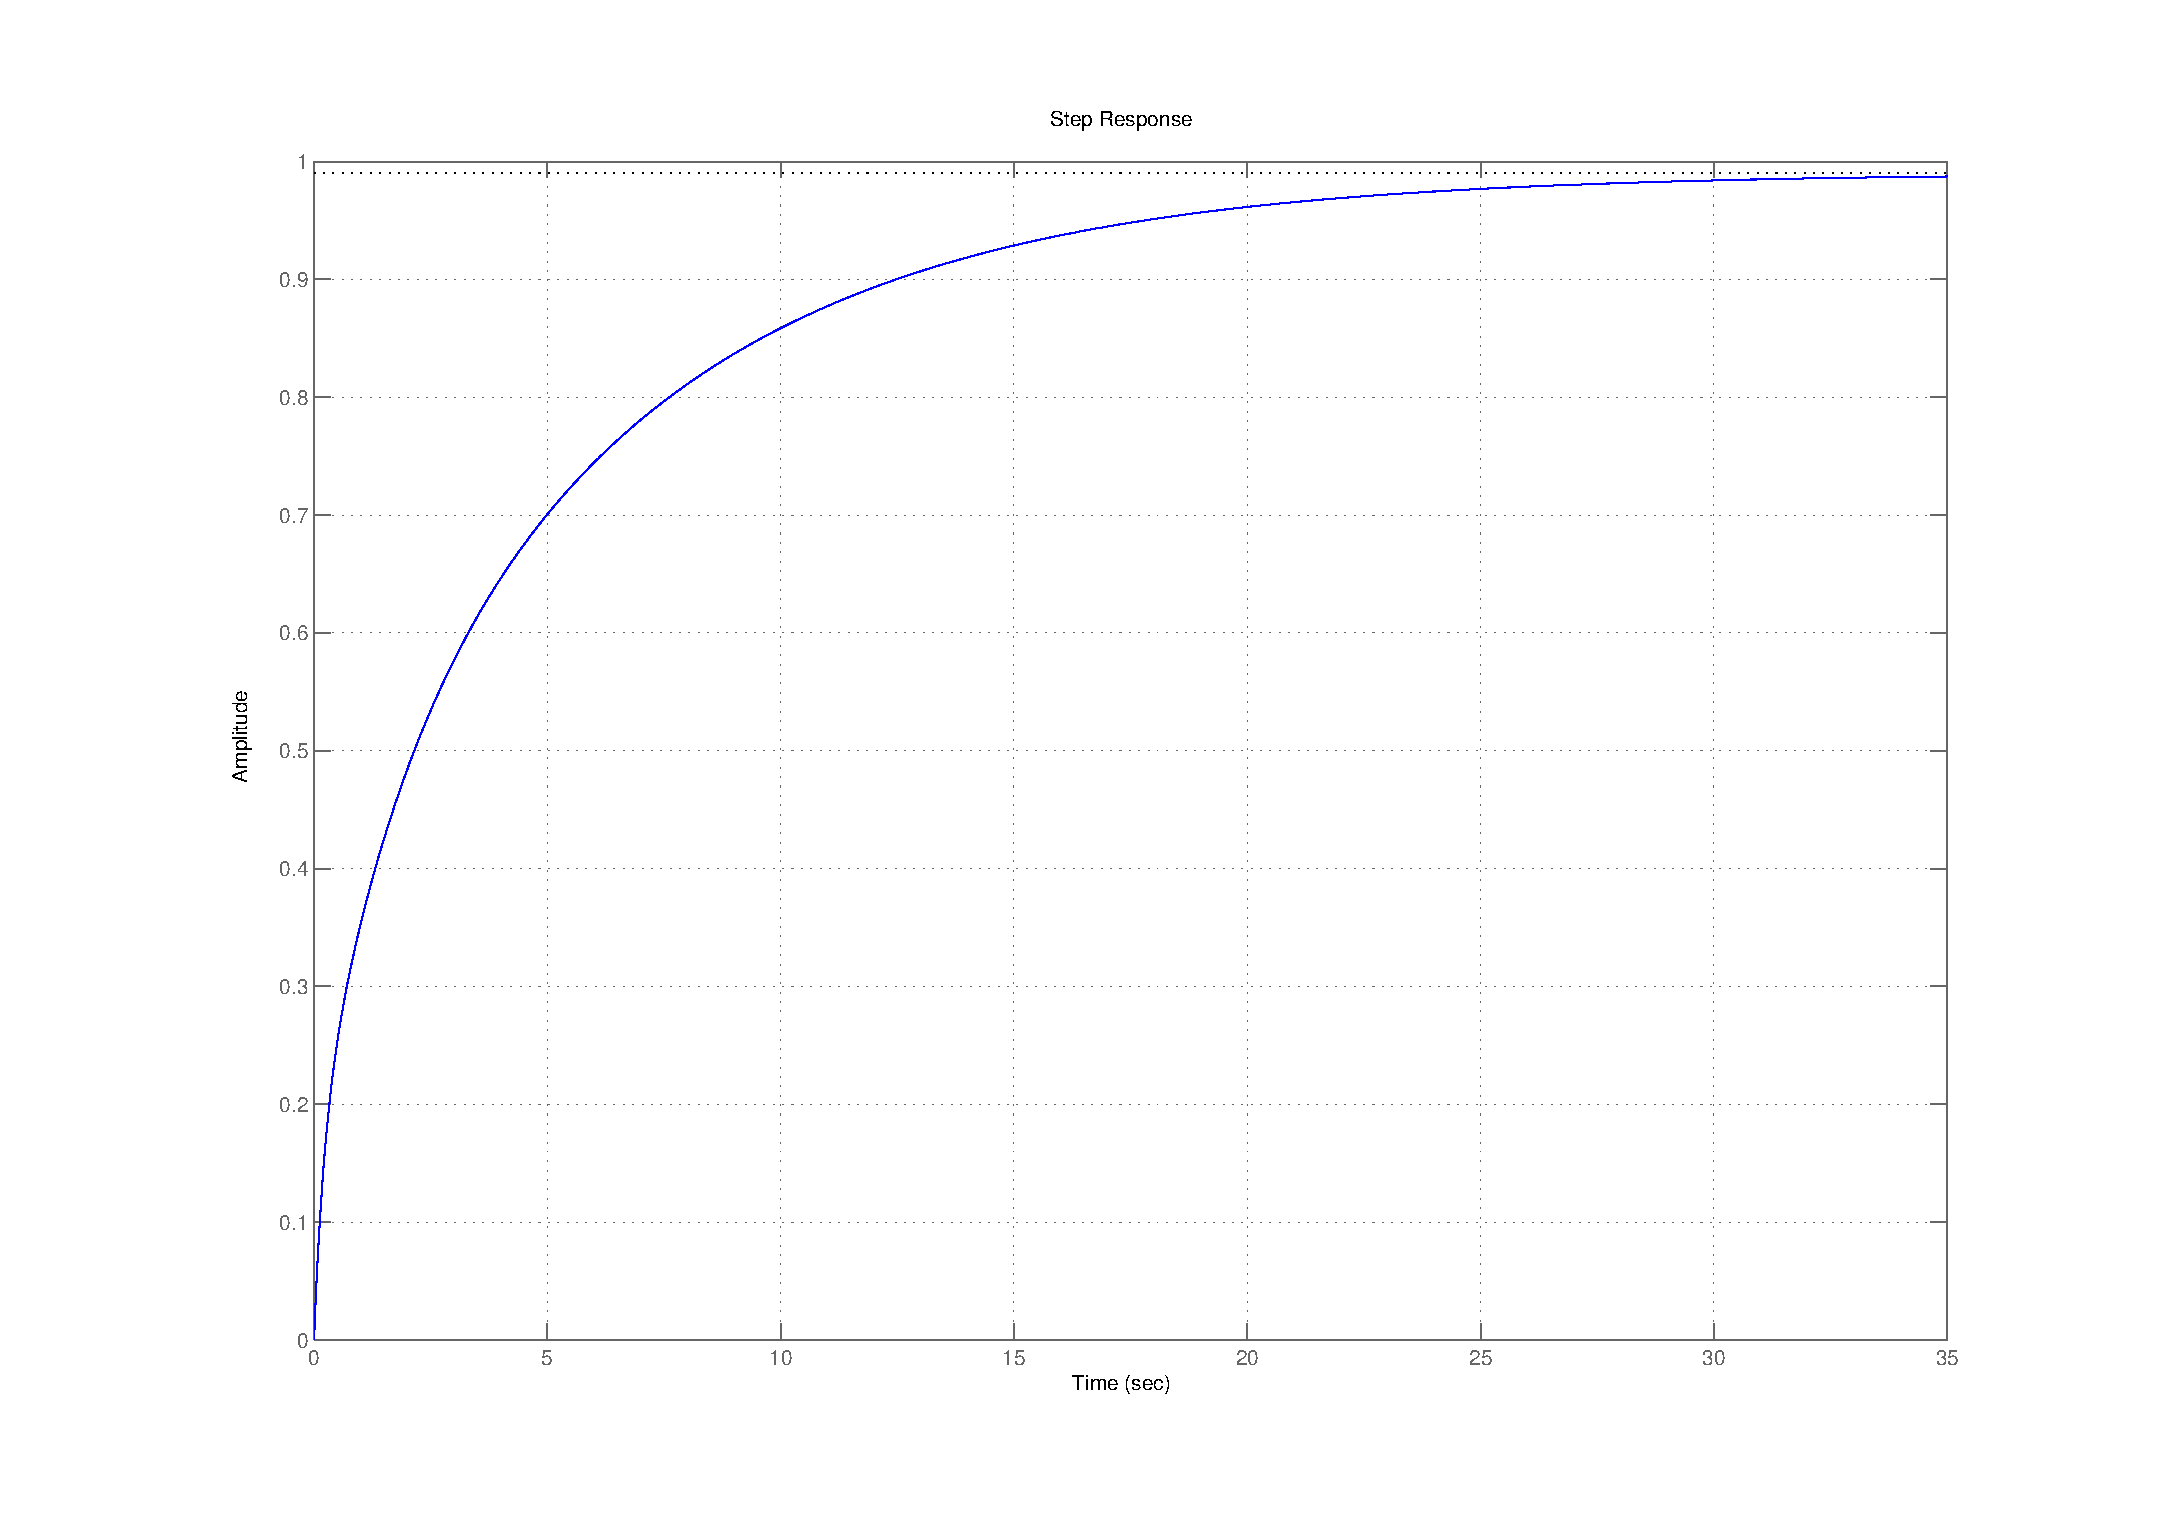
\includegraphics[width=0.95\textwidth]{imgs/questao2/resposta_gcomp1}
\caption{Resposta ao degrau para o controlador $G_c(s) = \frac{s+0,3}{s+0,0022}$}
\label{fig:q2:resposta_gcomp1}
\end{figure}

Analisando a figura observa-se que o desempenho do regime permanente tende para
o valor desejado (próximo a 1). Contudo, o tempo de subida do sistema pode vir a
ser um problema, repare a escala do tempo em comparação ao sistema em malha
fechada sem o controlador analisado na Fig. \ref{fig:q2:resposta_gmf}. Assim
sendo, observando o lugar geométrico das raízes do sistema com compensador,
mostrado na Fig. \ref{fig:q2:rlocus_gcomp1}, com o intuito de melhorar o
desempenho do tempo de subida, aumentou-se o ganho do sistema, distanciando os
polos do eixo imaginário. Para um ganho $k_c = 20$ foi obtida a resposta dada
pela Fig. \ref{fig:q2:resposta_gcomp2}.

\begin{figure}[H]
\centering
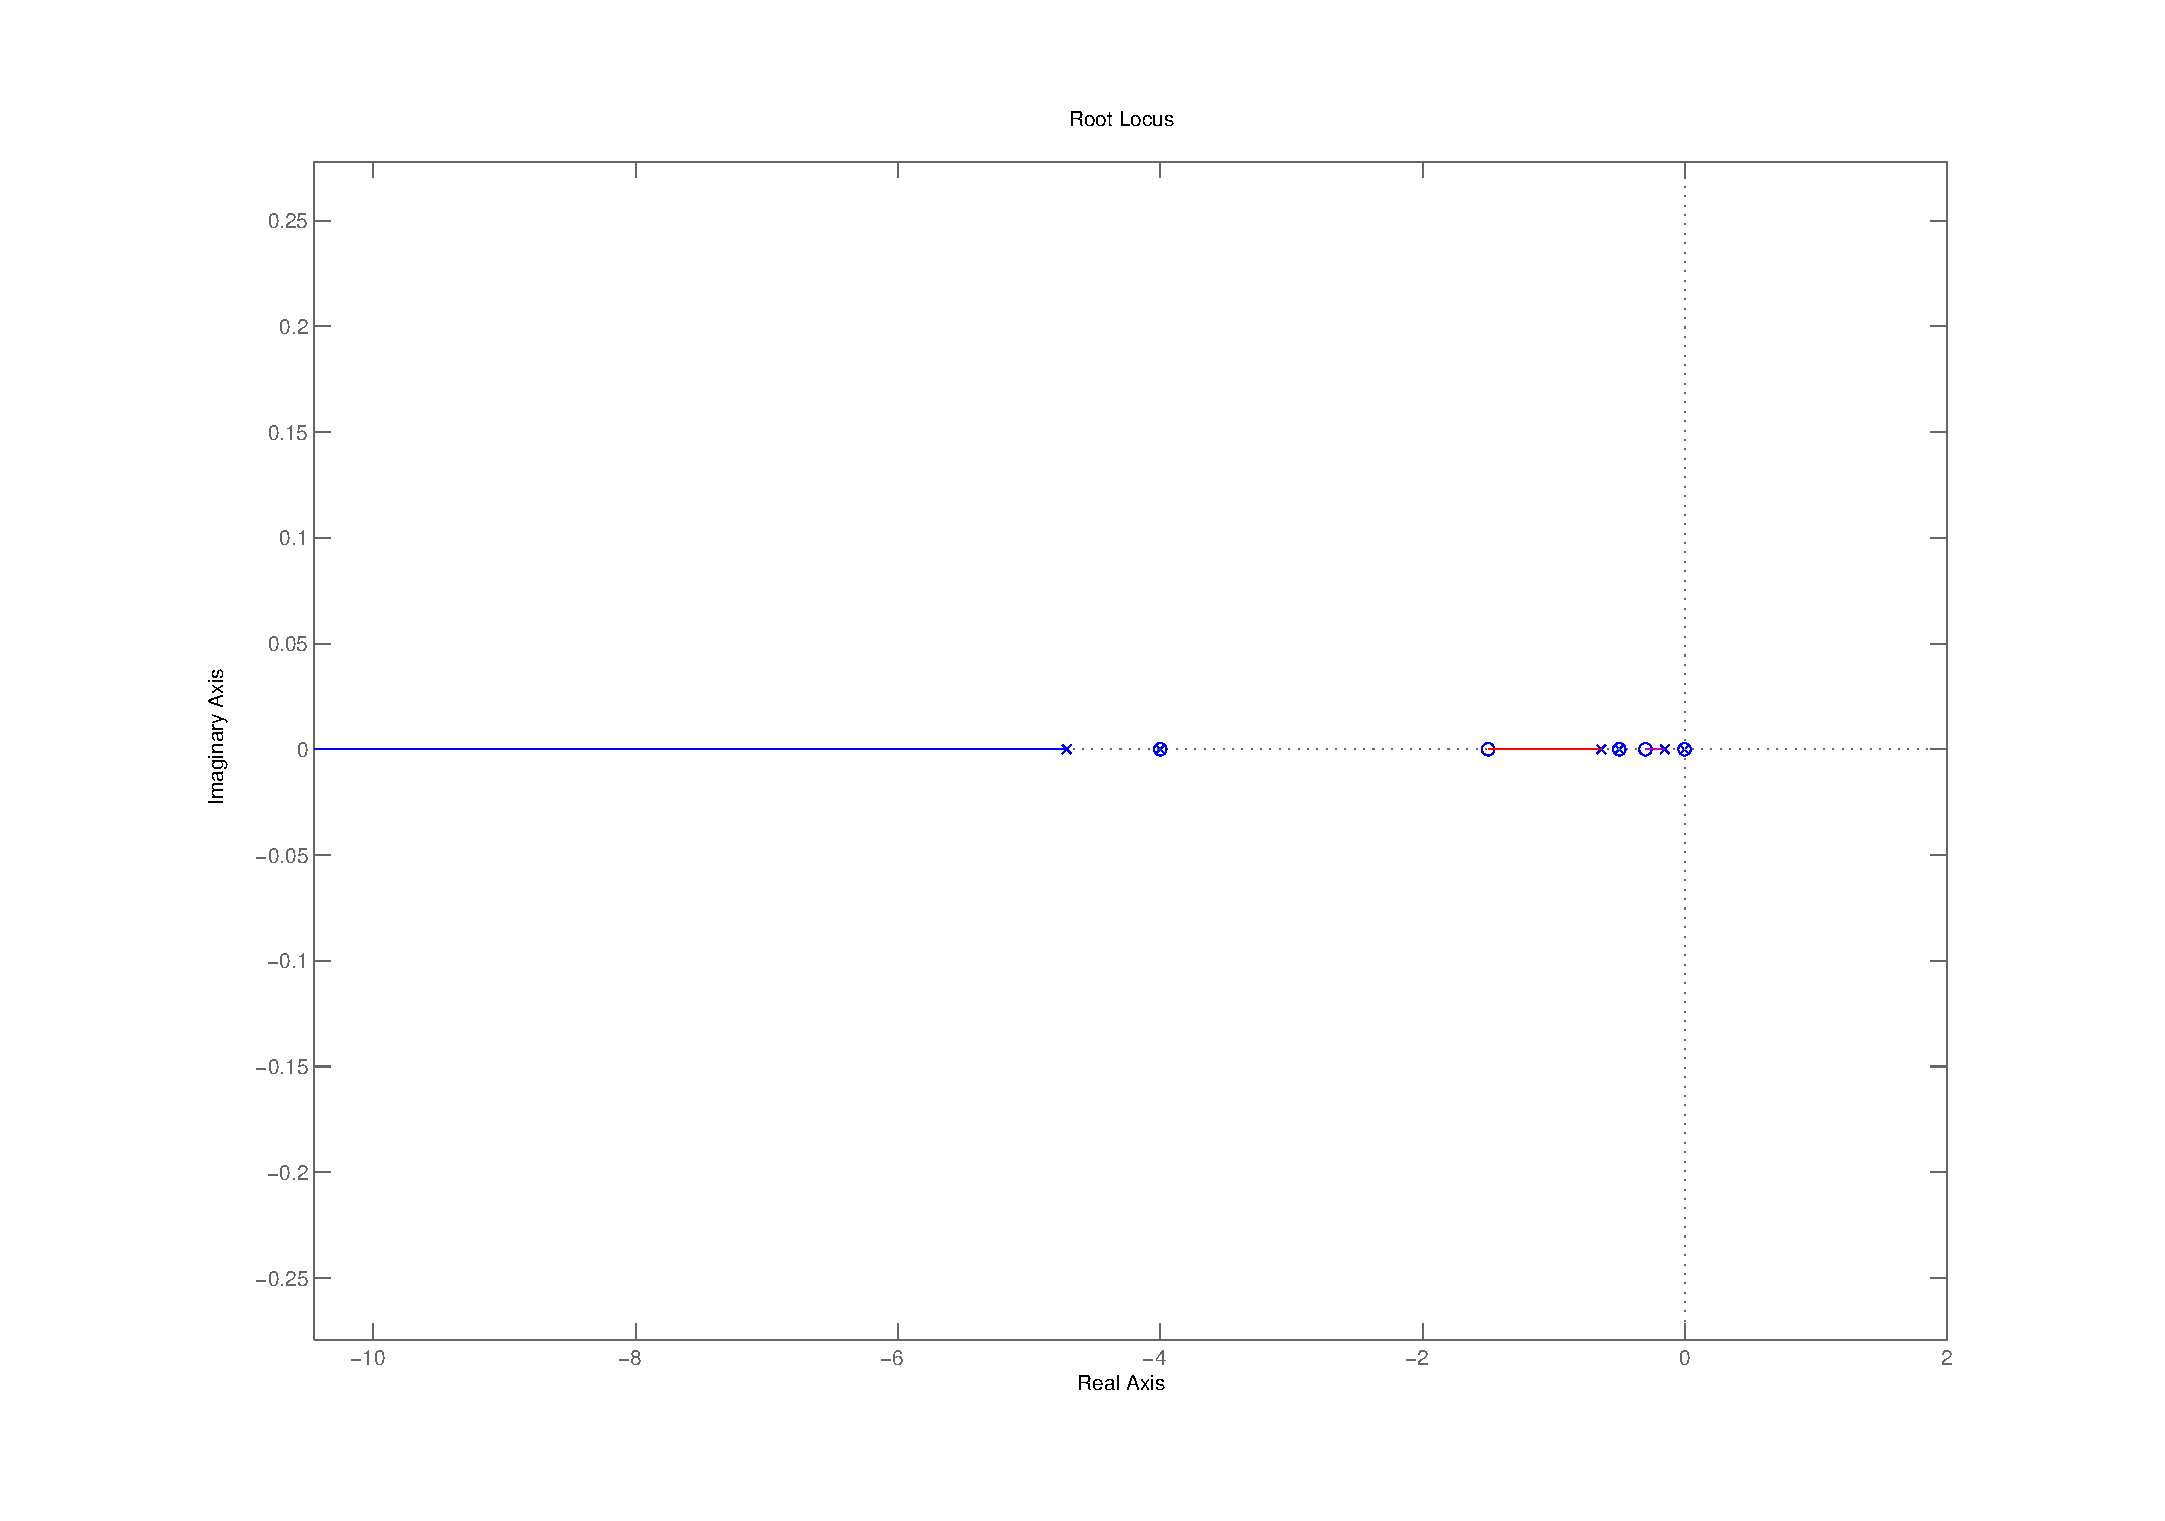
\includegraphics[width=0.95\textwidth]{imgs/questao2/rlocus_gcma}
\caption{Lugar das raízes para o sistema com o controlador $G_c(s)$}
\label{fig:q2:rlocus_gcomp1}
\end{figure}
 
\begin{figure}[H]
\centering
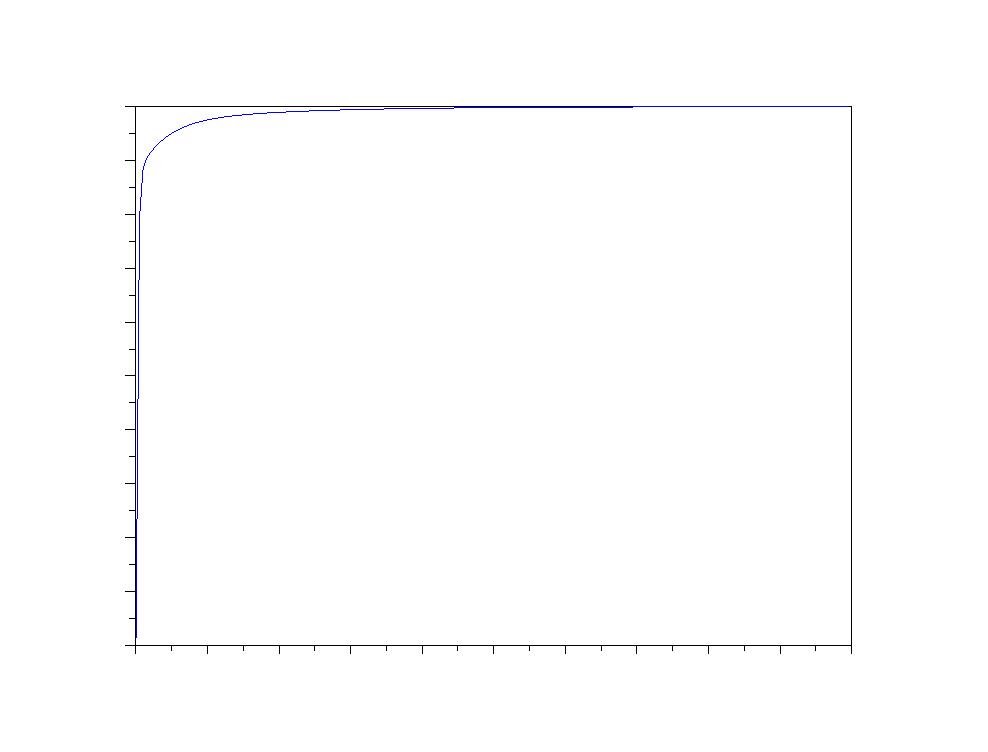
\includegraphics[width=0.95\textwidth]{imgs/questao2/resposta_gcomp2}
\caption{Reposta do sistema com o controlador $G_c(s) = 20\frac{s+0,3}{s+0,0022}$ }
\label{fig:q2:resposta_gcomp2}
\end{figure}

Percebe-se facilmente que há uma melhora substancial no tempo de subida do
sistema. A estabilidade do sistema para o novo valor de $k_c$ foi testada mais
uma vez através dos polinômios de Kharitonov, obtendo os seguintes valores:

\begin{flalign*}
q_1 & = 0.3+26.0066s+26.0022s^{2}+s^{3} \\
q_2 & = 0.3+51.0132s+26.0022s^{2}+s^{3} \\
q_3 & = 0.611+26.0066s+24.0022s^{2}+s^{3} \\
  q_4 & = 0.611+51.0132s+24.0022s^{2}+s^{3}
\end{flalign*}

\noindent e as suas raízes:

\begin{flalign*}
\begin{matrix}
q_1(s) & q_2(s) & q_3(s) & q_4(s) \cr
-0.012&-0.006&-0.024&-0.012\cr -1.03&-2.131&-1.112&-2.343\cr
-24.961&-23.865&-22.866&-21.647\cr 
\end{matrix}
\end{flalign*}

Uma vez que o sistema é estável na faixa de variação dos parâmetros de $G(s)$, o
controle é robusto. Como a resposta de regime transitório e permanente é
satisfatória, o controlador em atraso de fase foi suficiente para o projeto do
sistema. Assim sendo a parte em avanço de fase não foi projetada. O controlador
projetado é, portanto:

\begin{flalign*}
G_c(s) = 20\frac{s+0.3}{s+0.0022}
\end{flalign*}

Os {\it scripts} do \Matlab desenvolvidos para a resolução dessa questão podem
ser encontrados no Apêndices \ref{ap:cod_q2_kharitonov_a} a
\ref{ap:cod_q2_simulacao}.

% TODO(crisgc): Colocar o desempenho do controlador para alguns valores
% "randômicos" da função de transferência
